\section{Risultati}
Vengono riportati alcuni risultati di esempio ottenuti eseguendo il programma:
\newline \newline

Binary digits of log2 starting at position 1: 10110001

Binary digits of log2 starting at position 100: 00011111

Binary digits of log2 starting at position 10000: 00101101

Binary digits of log2 starting at position 1000000: 11010100

Binary digits of log2 starting at position 100000000: 01100111
\newline \newline

Hexadecimal digits of pi starting at position 1: 243F6A88

Hexadecimal digits of pi starting at position 100: C29B7C97

Hexadecimal digits of pi starting at position 10000: 68AC8FCF

Hexadecimal digits of pi starting at position 1000000: 26C65E52

Hexadecimal digits of pi starting at position 10000000: 17AF5863

\subsection{Tempo di computazione}
Sperimentalmente si può vedere come il tempo di calcolo sia piuttosto lineare rispetto a \textit{n}.

Infatti i tempi necessari per ricavare i risultati precedenti, sul mio laptop, sono rappresentati nel grafico che segue:

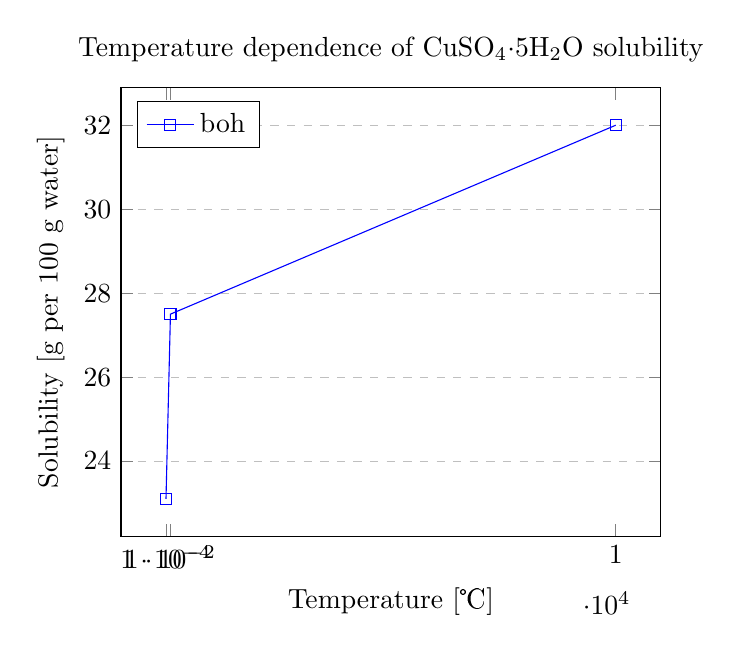
\begin{tikzpicture}
\begin{axis}[
%     width=\textwidth,
    title={Temperature dependence of CuSO$_4\cdot$5H$_2$O solubility},
    xlabel={Temperature [\textcelsius]},
    ylabel={Solubility [g per 100 g water]},
    xtick={1,100,10000},
    legend pos=north west,
    ymajorgrids=true,
    grid style=dashed,
]
 
\addplot[
    color=blue,
    mark=square,
    ]
    coordinates {
    	(1,23.1)(100,27.5)(10000,32)
    };
    \legend{boh}
 
\end{axis}
\end{tikzpicture}

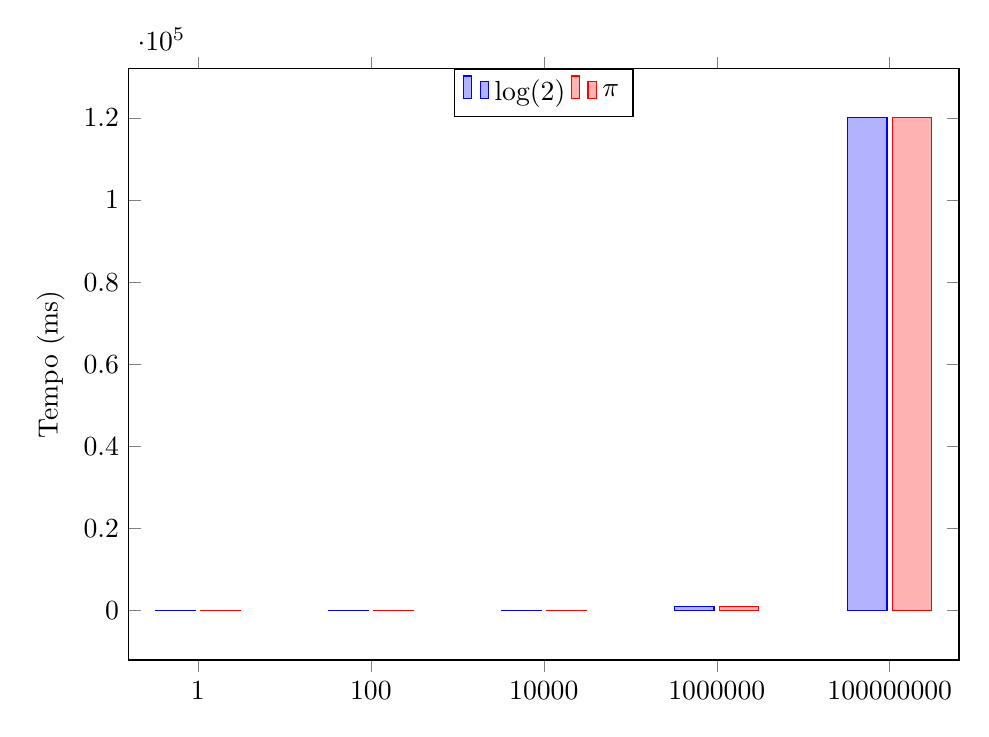
\begin{tikzpicture}
    \begin{axis}[
            ybar,
            bar width=.5cm,
            width=\textwidth,
            height=.75\textwidth,
            legend style={at={(0.5,1)},
                anchor=north,legend columns=-1},
            symbolic x coords={1,100,10000,1000000,100000000},
            xtick=data,
            ylabel={Tempo (ms)},
        ]
\addplot 
	coordinates {(1,0.474) (100,0.962) (10000,31.1)
		(1000000,1106) (100000000,120000)};
\addplot 
	coordinates {(1,0.474) (100,0.962) (10000,31.1)
		(1000000,1106) (100000000,120000)};
\legend{log(2),$\pi$}
\end{axis}
\end{tikzpicture}

\subsection{Possibili (futuri) utilizzi}
Partendo dal fatto che le cifre in $\pi$ \textbf{sembrano}\footnote{Non è stato dimostrato per il momento.} comparire equiprobabilmente, si potrebbe dedurre che prima o poi sia possibile incontrare qualunque sequenza di cifre.

Per questo motivo si può pensare di codificare un file, che non è altro che una sequenza di cifre, \textit{all'interno} di $\pi$.
Sarebbe sufficiente memorizzare solo la posizione della cifra iniziale e la sua lunghezza, recuperarlo usando il calcolo dell'n-sima cifra sarebbe poi \textit{relativamente facile}.

\noindent Sebbene per il momento il calcolo richiederebbe troppo tempo rendendo questa tecnica inutilizzabile, riporto i dati ottenuti sulla frequenza di comparsa di ciascuna cifra all'interno del primo milione di cifre:
\newline \newline
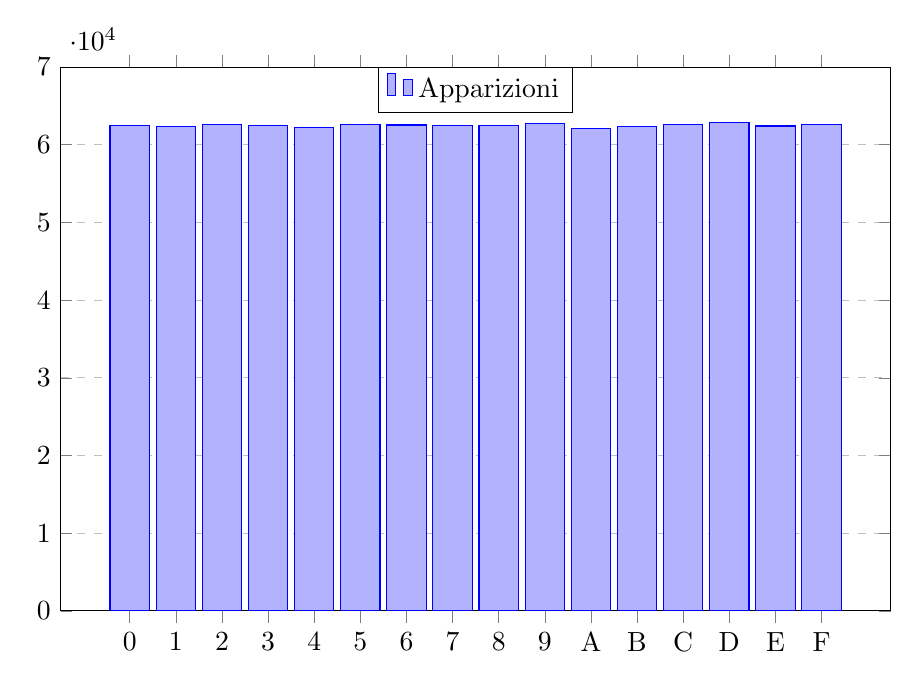
\begin{tikzpicture}
\begin{axis}[
ybar,
bar width=.5cm,
width=\textwidth,
height=.70\textwidth,
ymin=0, ymax=70000,
ymajorgrids=true,
grid style=dashed,
symbolic x coords={0,1,2,3,4,5,6,7,8,9,A,B,C,D,E,F},
xtick=data,
legend style={at={(0.5,1)},
anchor=north,legend columns=-1},
]
\addplot 
coordinates {(0,62522) (1,62385) (2,62644) (3,62432) (4,62235) (5,62649) (6,62545) (7,62515) (8,62459) (9,62699) (A,62070) (B,62345) (C,62621) (D,62829) (E,62415) (F,62635)};
\legend{Apparizioni}
\end{axis}
\end{tikzpicture}

Risulta evidente che ogni cifra appare più o meno equiprobabilmente, quindi forse in futuro ci saranno risvolti reali sull'utilizzo di una costante come il Pi greco per la codifica di file.